\section{Projeto}
Para a construção do nosso projeto optamos a linguagem C\# pela facilidade e infinidade de recursos para esse tipo de aplicação. A construção do projeto foi feita na IDE Visual Studio com os recursos providos do software.

Para melhorar a usabilidade criamos algumas telas para facilitar a interação do usuário com o software.

\begin{figure}[!htb]
	\centering
	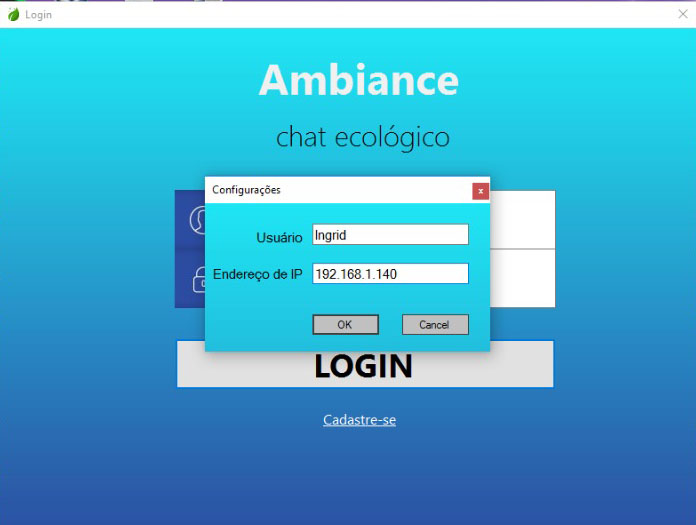
\includegraphics[scale=0.4]{img/t-conectar.jpeg}
	\caption{Tela de configurações}
	\label{Tela de configurações}
\end{figure}

\begin{figure}[!htb]
	\centering
	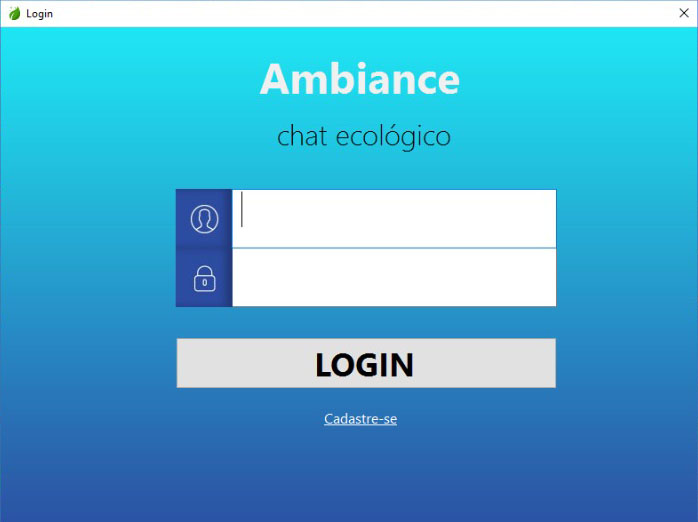
\includegraphics[scale=0.4]{img/t-login.jpeg}
	\caption{Tela de login}
	\label{Tela de login}
\end{figure}

\begin{figure}[!htb]
	\centering
	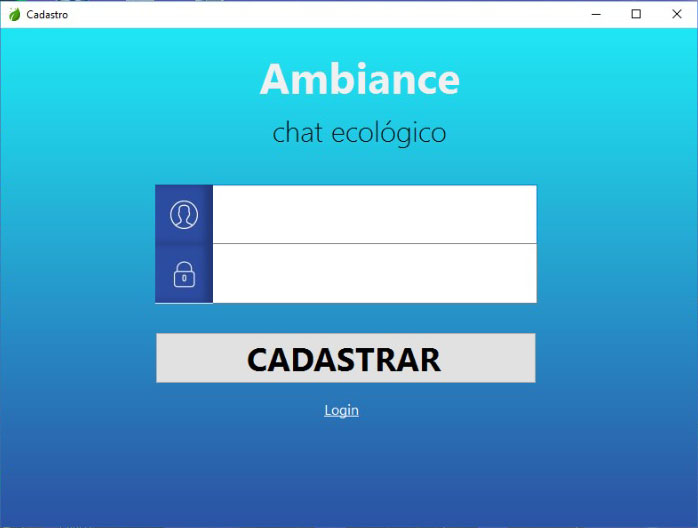
\includegraphics[scale=0.4]{img/t-pag-cadastro.jpeg}
	\caption{Tela de cadastro}
	\label{Tela de cadastro}
\end{figure}

\begin{figure}[!htb]
	\centering
	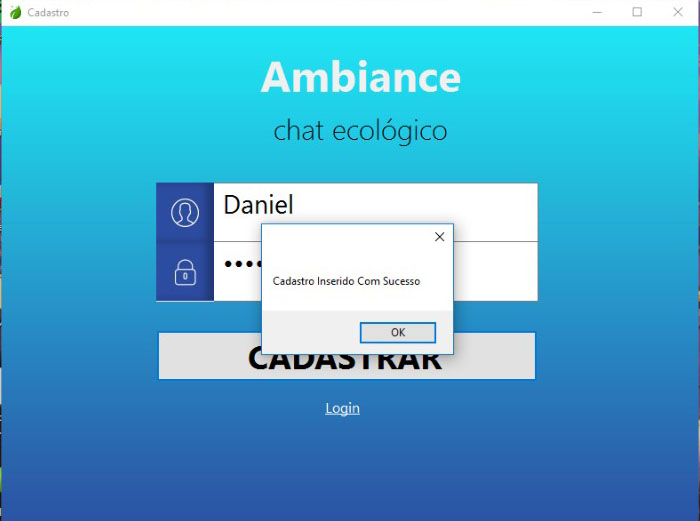
\includegraphics[scale=0.4]{img/t-cadastro-sucesso.jpeg}
	\caption{Tela de cadastro inserido com sucesso}
	\label{Tela de cadastro inserido com sucesso}
\end{figure}

\begin{figure}[!htb]
	\centering
	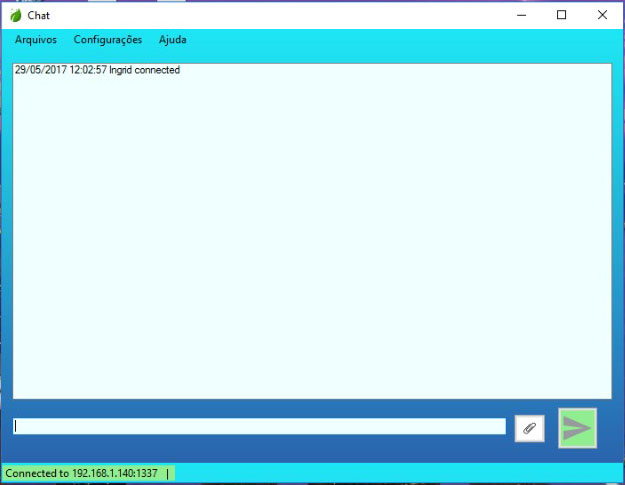
\includegraphics[scale=0.4]{img/t-rodando.jpeg}
	\caption{Aplicação em funcionamento}
	\label{Aplicação em funcionamento}
\end{figure}

\begin{figure}[!htb]
	\centering
	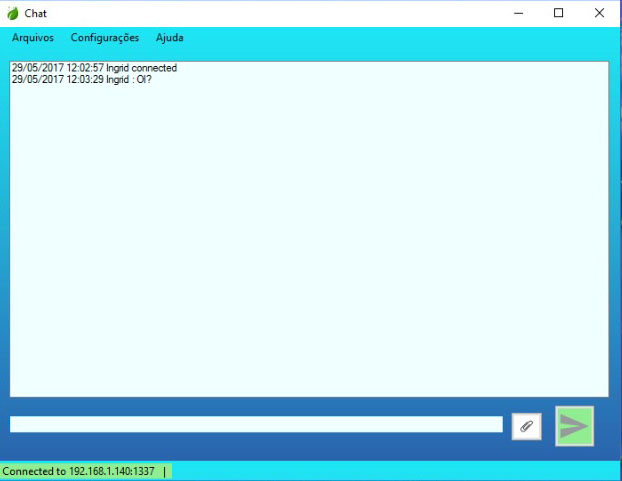
\includegraphics[scale=0.4]{img/t-msg-enviada.jpeg}
	\caption{Mensagem enviada}
	\label{Mensagem enviada}
\end{figure}

\begin{figure}[!htb]
	\centering
	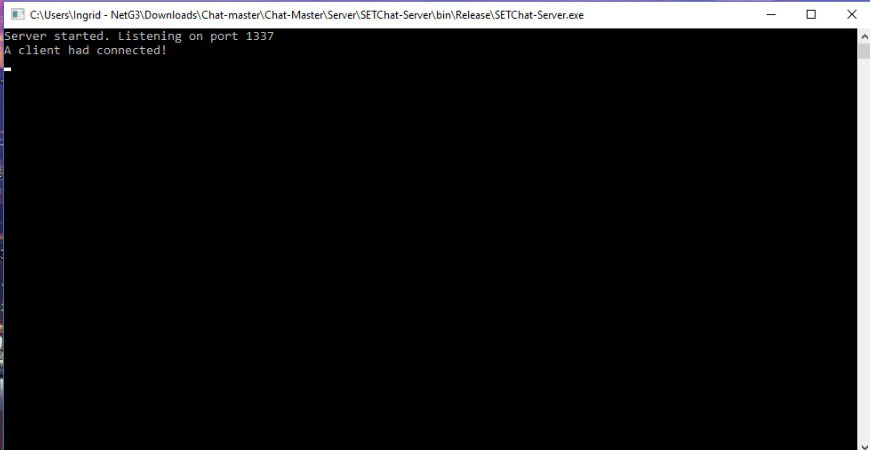
\includegraphics[scale=0.4]{img/t-log-server.jpeg}
	\caption{Log do servidor quando cliente se conecta}
	\label{Log do servidor quando cliente se conecta}
\end{figure}

\begin{figure}[!htb]
	\centering
	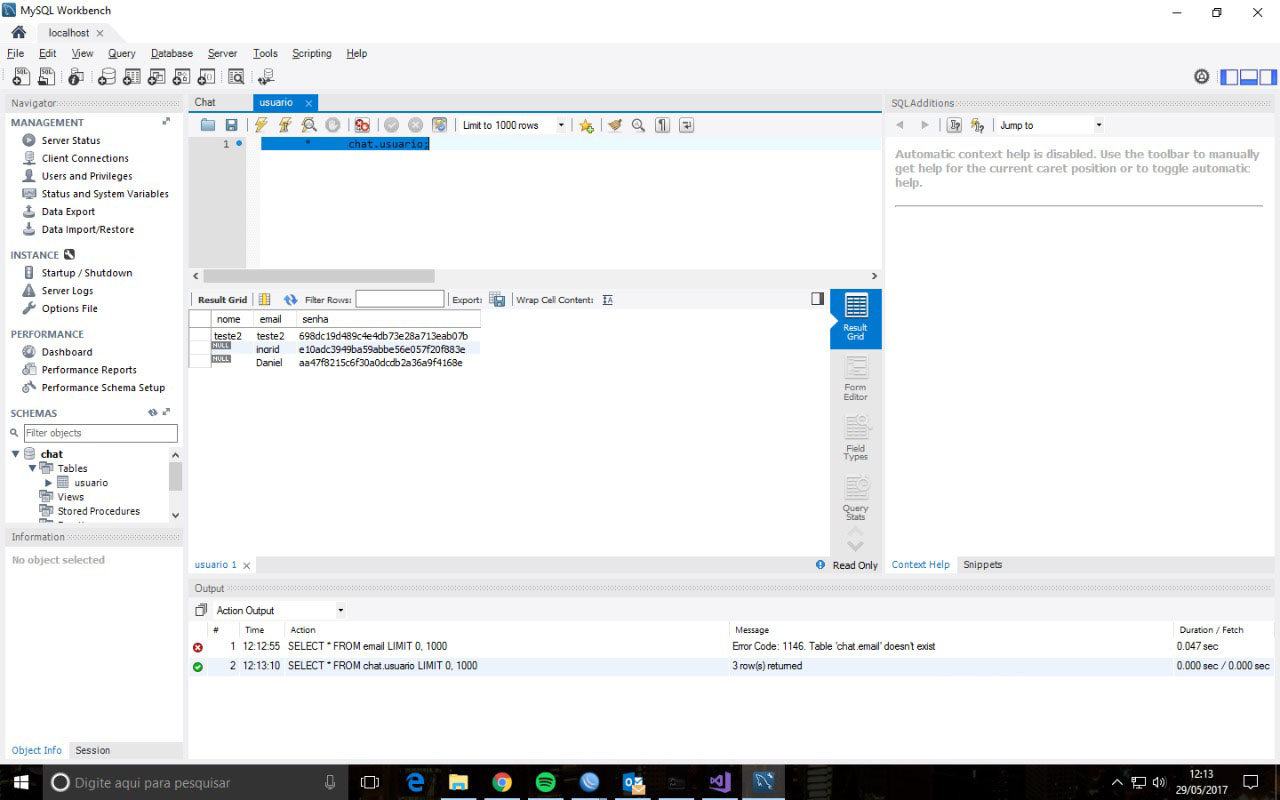
\includegraphics[scale=0.25]{img/t-banco-senha-cripto.jpeg}
	\caption{Tabela de senha do banco de dados criptografada com MD5}
	\label{Tabela de senha do banco de dados criptografada com MD5}
\end{figure}

